\chapter{Pathfinding}\label{ch:path}
Pathfinding is generally the process of finding a path from a given starting point ('A')
to a given destination ('B'),
on a given map.

There are different approaches to find the best path,
and different qualifiers for 'best'.

We chose to define 'best' as 'shortest time',
because in a real world application time is the most crucial resource in rescue.
In other applications 'best' could also mean shortest distance, least expensive (toll roads),
most convenient or any number of other qualifiers.

Since our robot has approximately equal movement speed in all used directions,
the shortest distance path will be very close to the shortest time path.
Since our robot only operates on a very limited map,
the shortest distance was also easiest to evaluate.

We chose to start implementing Dijkstra's shortest path algorithm,
since it is fairly simple to understand
and can be used as a baseline for better, more complicated algorithms,
like A*.

\section{Dijkstra}
Like with many others,
is the first step in Dijkstra's algorithm to reduce the map to the necessary minimum.
After this reduction, the map only consists of \emph{nodes} and \emph{edges}.
An edge connects two nodes together and has one integer \emph{travel cost}.
In this integer is stored how much it costs to traverse along that edge,
measured in the metric that should get optimized (in our case distance).

A node has a \emph{name}, an integer \emph{travel cost} and a reference to another node \emph{parent}.
The name is used as an identifier,
travel cost sums the travelling costs of all edges along the current shortest path
and parent refers to what node is the previous in that path.

\cite{Pound2017}

\begin{figure}[htp]
    \centering
    \subfloat[grid graph]{
        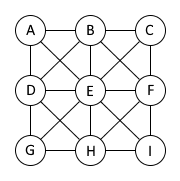
\includegraphics[width=0.24\textwidth]{figures/path/graph_grid}
    }
    \subfloat[circular graph]{
        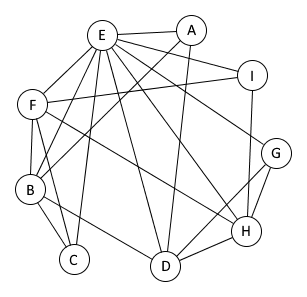
\includegraphics[width=0.24\textwidth]{figures/path/graph_circular}
    }
    \subfloat[tree graph]{
    	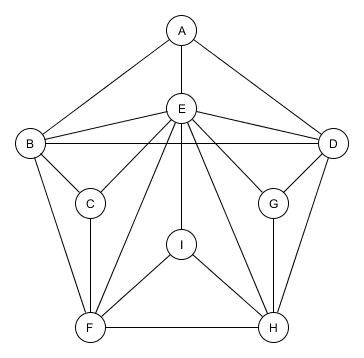
\includegraphics[width=0.24\textwidth]{figures/path/graph_tree}
    }
  	\subfloat[unstructured graph]{
  		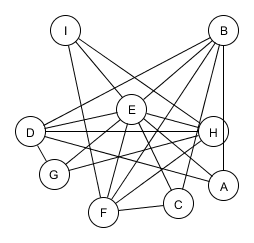
\includegraphics[width=0.24\textwidth]{figures/path/graph_unstructured}
	}
  	\caption{different representations of the same graph}
\end{figure}

%There also exists a list of all nodes, sorted by their travel cost, from low to high.

Dijkstra's approach now is to look at the facts we already know:
The shortest path from A to A
and the costs to get to any of A's neighbours.

Those values then get added to and stored  inside the neighbours' travel cost with A as the parent.
Now the starting node gets marked as done
and the node with the lowest travel cost gets selected
as the starting point for the next round of calculations

\todo{do we want this next paragraph?}
Since the only known travel cost before runtime is the starting node (being 0),
this is always where calculations start.

This algorithm can be implemented recursively,
with the starting point being the node with the lowest value
and the breaking condition of the starting pint being equal to the destination.

It can also be implemented to loop a given amount of times,
iterating through all existing nodes.

\section{Pathfinding on a grid}
Pathfinding on a grid is slightly different to pathfinding on a regular map,
because all nodes tend to have the same amount of neighbours,
and all edges have the same or similar costs.
\begin{figure}[htp]
	\centering
	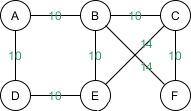
\includegraphics[width=0.24\textwidth]{figures/path/graph_values}
	\caption{3x3 grid with edge costs}
	\label{fig:graph_cost}
\end{figure}
%\missingfigure{closeup of a grid map, with values}


\section{Our implementation}
\todo[inline]{does this belong into sec:map-handle?}
For our grid we chose to allow vertical, horizontal and diagonal movement,
giving us 8 possible directions to move in from every node.
We decided to store those eight directions in one single byte,
with the least significant nibble (LSN) corresponding to the four main directions (N,E,S,W),
and the MSN corresponding to NE, SE, SW and NW.

\begin{center}
	\begin{tabular}{|*{8}{m{0.6cm}|}|l|}
		\hline
		N & E& S& W& NE& SE& SW& NW& byte\\
		\hline
		0 & 0 & 0 & 0 & 0 & 0 & 0 & 1 & 0x01\\
		0 & 0 & 0 & 0 & 0 & 0 & 1 & 0 & 0x02\\
		0 & 0 & 0 & 0 & 0 & 0 & 1 & 1 & 0x03\\
		0 & 0 & 0 & 0 & 1 & 1 & 1 & 0 & 0x\\
		\hline
		1 & 0 & 1 & 0 & 1 & 0 & 1 & 0 & 0x\\
		1 & 0 & 1 & 0 & 1 & 0 & 1 & 0 & 0x\\
		1 & 0 & 1 & 0 & 1 & 0 & 1 & 0 & 0x\\
		1 & 0 & 1 & 0 & 1 & 0 & 1 & 0 & 0x\\
		\hline
	\end{tabular}
\end{center}

%\missingfigure{maybe a table would be better. hex values for directions}


\todo{fix citation stuff}
\cite{Madsen2010}, \cite{Oetiker2010} and \cite{Mittelbach2005}.
